\documentclass[12pt]{article}
%\documentclass{article}

\usepackage{times}
\usepackage[final]{graphicx}
\usepackage{hyperref}

\setlength{\topmargin}{-0.5in}
\setlength{\oddsidemargin}{0in}
\setlength{\evensidemargin}{0in}
\setlength{\textwidth}{6.5in}
\setlength{\textheight}{9.0in}

\begin{document}

\centerline{\bf \Large CS295/CS395/CSYS395: \href{CS295_395_Syllabus.pdf}{\underline{Evolutionary Robotics}}}

\vspace{0.5cm}

\centerline{\bf \large Programming Assignment 10 of 10}

\vspace{0.5cm}

\centerline{\large Assigned: Monday, November 4, 2011}

\vspace{0.5cm}

\centerline{\large Due: Monday, November 11, 2011 by midnight}

\vspace{0.5cm}

\noindent \textbf{Description:} In this assignment you will integrate the evolutionary algorithm you developed in Python with the robot simulator. This requires six steps:

\begin{enumerate}
\item From the Python code copied from assignment 3, output a matrix of synaptic weights to a text file.
\item When the ODE code starts, it creates the robot, reads in this matrix, and sets the synaptic weights from the sensors to the motors.
\item The ODE code runs for 1000 time steps, after which the robot's displacement from the origin is written into a text file.
\item This number is read in by the Python code, and assigned as the fitness of the parent synaptic weight matrix.
\item A mutated, child synaptic weight matrix is created and sent to the ODE simulation.
\item In ODE the robot's position is set back to the origin, the new synaptic weights are read in, and so on.
\end{enumerate}

\begin{figure}
\centerline{
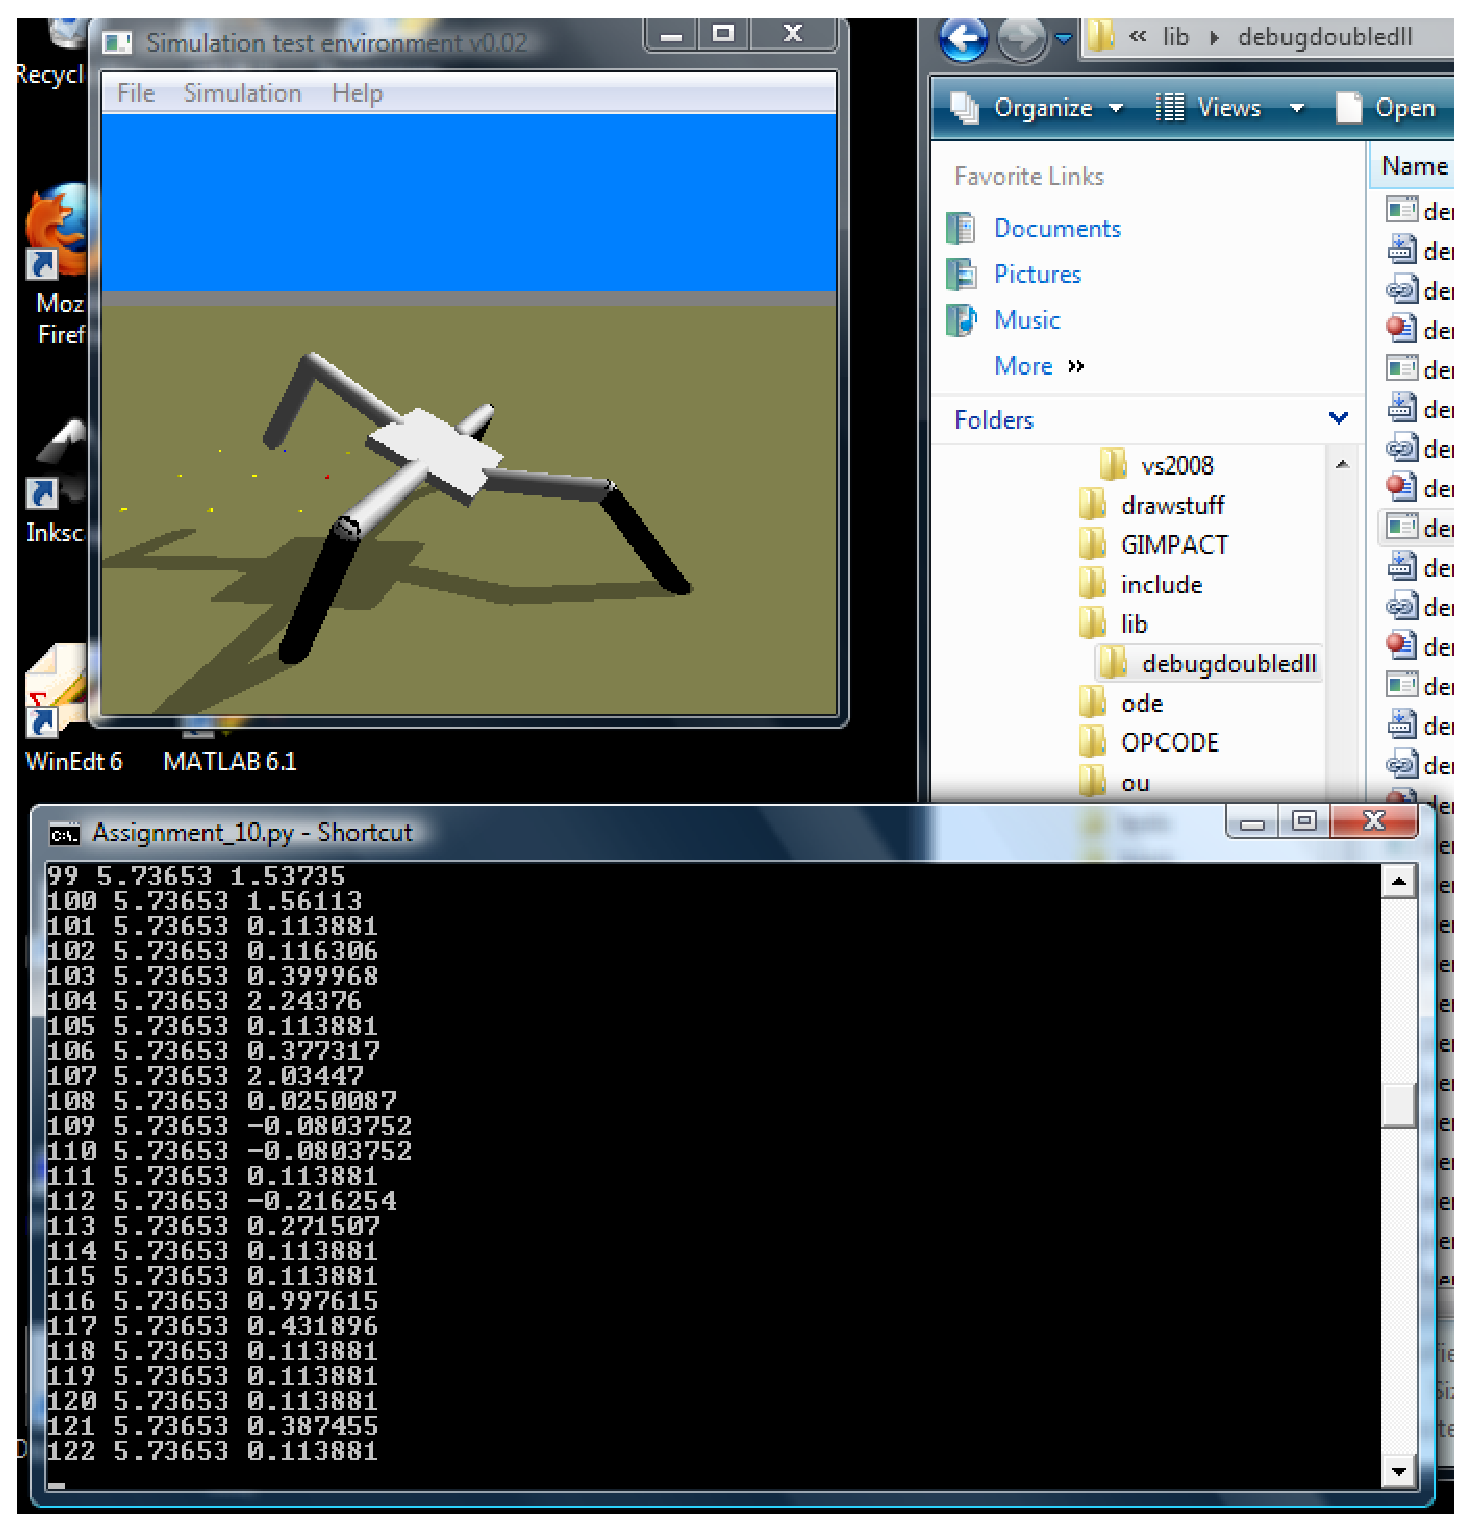
\includegraphics[width=1.0\textwidth]{Fig1.eps}}
\caption{Display of the robot's behavior (graphics window) and the evolutionary algorithm running in Python (text window).}
\label{Fig1}
\end{figure}

These steps are to be realized as follows.

\begin{enumerate}

\item Back up Assignment\_9 on a flash drive or another computer so that you can always return to your completed eighth assignment.

\item Copy directory Assignment\_9, which contains your submitted document and the entire ODE folder. Rename the new directory Assignment\_10.

\item Copy the Python code you created in assignment 3 into this new directory.

\item In the Python code, change the dimension of the synaptic weight matrices so that they are $4 \times 8$, and ensure that the values range in $[-1,1]$.

\item After the parent matrix is created, write out the matrix to a text file called \texttt{weights.dat}. Make sure this file is stored in the directory where your ODE simulation will run. This directory is usually \texttt{ode-0.11.1$\backslash$lib$\backslash$debugdoubledll} on a Windows machine, but will be different on other platforms.

\item The Python code should then periodically check for the existence of the second file, which will report the fitness of the parent matrix. You can implement this using the \texttt{path.os.exists} and \texttt{sleep} Python functions: \\
   \texttt{fileName = 'fit.dat';}\\
   \texttt{while ( os.path.exists(fileName)==False ):}\\
.\hspace{0.5cm}\texttt{\hspace{0.5cm}sleep(0.2);}\\

 \item Once this part of the Python code is working, set it aside. In the ODE simulation, create a new variable \texttt{timer} that is set to zero, and incremented during each pass through \texttt{simLoop} when it is unpaused.

 \item When the timer reaches 1000---that is, 1000 iterations through \texttt{simLoop} have been performed---set the timer to zero again. Also, reset the robot by destroying all of its body parts and joints, and recreating them at the origin: \\
   \texttt{internalTimer++;}\\
   \texttt{if ( internalTimer == 1000 ) \{}\\
.\hspace{0.5cm}\texttt{internalTimer = 0;}\\
.\hspace{0.5cm}\texttt{DeleteRobot();}\\
.\hspace{0.5cm}\texttt{CreateRobot();}\\
   \texttt{\}}\\

\item Run the ODE code; you should see the robot performing the same behavior repeatedly for 1000 time steps. This is because you are not resetting the synaptic weight matrix yet.

\item Add an additional line to \texttt{CreateRobot()}\\
\texttt{WeightsRead()}\\
that looks for the text file \texttt{weights.dat}. Once it exists, it reads in the values and stores them in the matrix \texttt{weights} that you created in the last assignment. Finally, this function deletes the file. Check any online C tutorial to learn how to check whether a file exists, and how to delete it. When you run the ODE simulation now, it should simulate the robot once, and then freeze, because when it gets to the \texttt{if} clause in \texttt{simLoop} when \texttt{CreateRobot} is called for the second time, there is no file for it to read in.

\item Now add an additional line that calls a function \texttt{Fitness\_Save()} to the \texttt{if} clause \\
   \texttt{internalTimer++;}\\
   \texttt{if ( internalTimer == 1000 ) \{}\\
.\hspace{0.5cm}\texttt{internalTimer = 0;}\\
.\hspace{0.5cm}\texttt{Fitness\_Save();}\\
.\hspace{0.5cm}\texttt{DeleteRobot();}\\
.\hspace{0.5cm}\texttt{CreateRobot();}\\
   \texttt{\}}\\
This function should get the position of the robot's main body using \\
\texttt{dBodyGetPosition()}\\
(see the ODE documentation). It should take the horizontal component of this final position, and write it to a text file \texttt{fit.dat}.

\item Run your ODE simulation, and make sure that it stores a single number in \texttt{fit.dat}. Now, update your Python code so that when the file \texttt{fit.dat} exists, it reads in the value, stores it in \texttt{parentFit}, and deletes the file. This can be done in Python using \\
\texttt{os.remove('fit.dat');}

\item In the Python code, once \texttt{parentFit} has been set and \texttt{fit.dat} has been deleted, a child matrix can be created, and its values stored in \texttt{weights.dat}. The Python code should then pause again until the fitness of the child matrix is returned by the ODE simulation. When it is, the Python code should print the current generation, the fitness of the parent, and the fitness of the child.

\item Now you should be able to run your Python code, and, while it is running, start up your ODE code. Make sure that the following actions occur in the right order: (1) the Python code outputs a weight matrix; (2) the ODE simulation reads in and deletes this matrix; (3) the ODE code simulates the robot's behavior while the Python code waits; (4) the ODE code saves the robot's fitness; (5) the Python code reads in this fitness and deletes the file; and (6) the Python code writes another synaptic weight matrix.

\item If your two applications communicate with one another correctly, you should see something like in Fig. \ref{Fig1}. The graphics window shows the behavior of the robot using the current synaptic weight matrix, and the text window corresponding to the Python code outputs the results of each `generation'.

\item Make sure to do a screencapture that captures both your robot in action and the results of your evolutionary algorithm after a few generations. The T.A. will look to verify two aspects of your screenshot. First, that when the child has a higher fitness than the parent (the third number in a row is higher than the second number in a row), the child becomes the parent (the third number in row $i$ becomes the second number in row $i+1$. Second, make sure to capture one of the better of the child solutions moving to the right: if you select for the horizontal component of the robot's final position, the robot should start to move to your right. Note how in Fig. \ref{Fig1} the robot is to the right of the dots at the left of the graphics window (these dots indicate the $(0,0,0)$ origin).

\item Do a screencapture until you get such a combined image. Copy it into your document and send it to the T.A.

\end{enumerate}

\end{document} 